% answers.tex —— 2023 年·全国乙卷·理科 · 参考答案与详细解析片段
% 由 tools/generate_projects.py 依来源总账自 2023/2023_数学真题_全国乙理_试题.md + 2023/2023_数学真题_全国乙理_解析正文.md + 2023/2023_数学真题_全国乙理_答案要点.md 生成，勿手改（改源 MD 后重跑）

\begin{gknotice}
\textbf{解析归属：}下列过程由本库依据固定原卷独立推导，\textbf{不是官方答案}，并经另一角色逐题盲核。
\end{gknotice}

\gkpart{一、单选题}

\begin{answer}
\gksolhead{1}{}

\textbf{题目}：

设 $z=\dfrac{2+\mathrm i}{1+\mathrm i^2+\mathrm i^5}$，则 $\overline z=$\mbox{（　　）}

\begin{gkopts}(4)
\task A．$1-2\mathrm i$
\task B．$1+2\mathrm i$
\task C．$2-\mathrm i$
\task D．$2+\mathrm i$
\end{gkopts}

\Needspace{4\baselineskip}
\textbf{解析}

\Needspace{5\baselineskip}
由 $\mathrm i^2=-1$、$\mathrm i^5=\mathrm i$，分母为

\nopagebreak[4]
\[
1+\mathrm i^2+\mathrm i^5=\mathrm i.
\]

所以 $z=(2+\mathrm i)/\mathrm i=1-2\mathrm i$，从而 $\bar z=1+2\mathrm i$，选 B。

\gkanswer{答案：B}

\end{answer}
\begin{answer}
\gksolhead{2}{}

\textbf{题目}：

设全集 $U=\mathbb R$，集合 $M=\{x\mid x<1\}$，$N=\{x\mid -1<x<2\}$，则 $\{x\mid x\geqslant2\}=$\mbox{（　　）}

\begin{gkopts}(2)
\task A．$\complement_U(M\cup N)$
\task B．$N\cup\complement_U M$
\task C．$\complement_U(M\cap N)$
\task D．$M\cup\complement_U N$
\end{gkopts}

\Needspace{4\baselineskip}
\textbf{解析}

$M\cup N=(-\infty,2)$，其在全集 $\mathbb R$ 中的补集为 $[2,+\infty)$，正是 $\{x\mid x\geqslant2\}$，选 A。

\gkanswer{答案：A}

\end{answer}
\begin{answer}
\gksolhead{3}{}

\textbf{题目}：

如图，网格纸上绘制的是一个零件的三视图，网格小正方形的边长为 $1$，则该零件的表面积为\mbox{（　　）}
\nopagebreak[4]
\begin{center}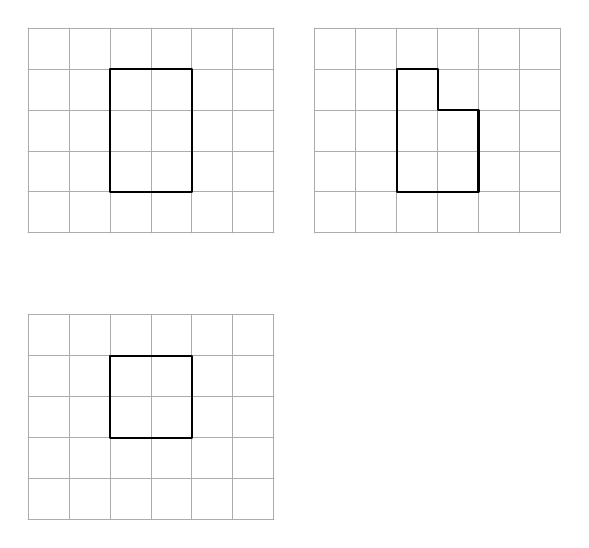
\begin{tikzpicture}[line cap=round,line join=round,line width=0.8pt,scale=0.52]
\begin{scope}[shift={(0,3)}]
  \draw[gray!65,line width=0.35pt] (0,0) grid (6,5);
  \draw[black] (2,1)--(4,1)--(4,4)--(2,4)--cycle;
\end{scope}
\begin{scope}[shift={(7,3)}]
  \draw[gray!65,line width=0.35pt] (0,0) grid (6,5);
  \draw[black] (2,1)--(4,1)--(4,3)--(3,3)--(3,4)--(2,4)--cycle;
\end{scope}
\begin{scope}[shift={(0,-4)}]
  \draw[gray!65,line width=0.35pt] (0,0) grid (6,5);
  \draw[black] (2,2)--(4,2)--(4,4)--(2,4)--cycle;
\end{scope}
\end{tikzpicture}
\end{center}
\nopagebreak[4]
\begin{gkopts}(4)
\task A．$24$
\task B．$26$
\task C．$28$
\task D．$30$
\end{gkopts}

\Needspace{4\baselineskip}
\textbf{解析}

\Needspace{5\baselineskip}
三视图显示零件可视为长度为 $2$ 的直棱柱，垂直于棱柱长度方向的截面是一个阶梯形：相邻两个单位宽条的高度分别为 $3$ 和 $2$。截面面积为 $3+2=5$，其边界周长为 $2+2+1+1+1+3=10$。棱柱表面积等于两个截面面积加侧面积：

\nopagebreak[4]
\[
S=2\cdot5+2\cdot10=30,
\]

选 D。

\gkanswer{答案：D}

\end{answer}
\begin{answer}
\gksolhead{4}{}

\textbf{题目}：

已知 $f(x)=\dfrac{xe^x}{e^{ax}-1}$ 是偶函数，则 $a=$\mbox{（　　）}

\begin{gkopts}(4)
\task A．$-2$
\task B．$-1$
\task C．$1$
\task D．$2$
\end{gkopts}

\Needspace{4\baselineskip}
\textbf{解析}

\Needspace{5\baselineskip}
对 $x\ne0$，

\nopagebreak[4]
\[
f(-x)=\frac{-xe^{-x}}{e^{-ax}-1}
=\frac{xe^{(a-1)x}}{e^{ax}-1}.
\]

函数为偶函数要求 $f(-x)=f(x)=xe^x/(e^{ax}-1)$ 对定义域内所有 $x$ 成立，故 $e^{(a-1)x}=e^x$，从而 $a=2$，选 D。

\gkanswer{答案：D}

\end{answer}
\begin{answer}
\gksolhead{5}{}

\textbf{题目}：

设 $O$ 为平面直角坐标系的坐标原点，在区域 $\{(x,y)\mid 1\leqslant x^2+y^2\leqslant4\}$ 内随机取一点，记该点为 $A$，则直线 $OA$ 的倾斜角不大于 $\dfrac\pi4$ 的概率为\mbox{（　　）}

\begin{gkopts}(4)
\task A．$\dfrac18$
\task B．$\dfrac16$
\task C．$\dfrac14$
\task D．$\dfrac12$
\end{gkopts}

\Needspace{4\baselineskip}
\textbf{解析}

\Needspace{5\baselineskip}
随机点在以原点为中心的圆环内均匀分布，极角在 $[0,2\pi)$ 上均匀。直线 $OA$ 的倾斜角按模 $\pi$ 计；倾斜角不大于 $\pi/4$ 对应总角度长度为 $2\cdot(\pi/4)=\pi/2$ 的两块扇形。因此概率为

\nopagebreak[4]
\[
\frac{\pi/2}{2\pi}=\frac14,
\]

选 C。

\gkanswer{答案：C}

\end{answer}
\begin{answer}
\gksolhead{6}{}

\textbf{题目}：

已知函数 $f(x)=\sin(\omega x+\varphi)$ 在区间 $\left(\dfrac\pi6,\dfrac{2\pi}3\right)$ 单调递增，直线 $x=\dfrac\pi6$ 和 $x=\dfrac{2\pi}3$ 为函数 $y=f(x)$ 的图象的两条对称轴，则 $f\left(-\dfrac{5\pi}{12}\right)=$\mbox{（　　）}

\begin{gkopts}(2)
\task A．$-\dfrac{\sqrt3}{2}$
\task B．$-\dfrac12$
\task C．$\dfrac12$
\task D．$\dfrac{\sqrt3}{2}$
\end{gkopts}

\Needspace{4\baselineskip}
\textbf{解析}

\Needspace{5\baselineskip}
正弦函数的对称轴是图象的极值轴，相邻两条相距半个周期。题给两轴距离为 $2\pi/3-\pi/6=\pi/2$，且函数在两轴之间递增，所以它们分别对应极小值轴和极大值轴，进而 $\pi/|\omega|=\pi/2$。无论以正还是负频率参数表示，在该区间上的函数都等价于

\nopagebreak[4]
\[
f(x)=\sin\left(2x-\frac{5\pi}{6}\right).
\]

\Needspace{5\baselineskip}
于是

\nopagebreak[4]
\[
f\left(-\frac{5\pi}{12}\right)
=\sin\left(-\frac{5\pi}{6}-\frac{5\pi}{6}\right)
=\sin\left(-\frac{5\pi}{3}\right)=\frac{\sqrt3}{2},
\]

选 D。

\gkanswer{答案：D}

\end{answer}
\begin{answer}
\gksolhead{7}{}

\textbf{题目}：

甲、乙两位同学从 $6$ 种课外读物中各自选读 $2$ 种，则这两人选读的课外读物中恰有 $1$ 种相同的选法共有\mbox{（　　）}

\begin{gkopts}(4)
\task A．$30$ 种
\task B．$60$ 种
\task C．$120$ 种
\task D．$240$ 种
\end{gkopts}

\Needspace{4\baselineskip}
\textbf{解析}

\Needspace{5\baselineskip}
先选甲读的两种书，有 $\binom62$ 种。乙要恰与甲有一种相同，需从甲选的两种中取一种（$2$ 种），再从甲未选的四种中取一种（$4$ 种）。总数为

\nopagebreak[4]
\[
\binom62\cdot2\cdot4=120,
\]

选 C。

\gkanswer{答案：C}

\end{answer}
\begin{answer}
\gksolhead{8}{}

\textbf{题目}：

已知圆锥 $PO$ 的底面半径为 $\sqrt3$，$O$ 为底面圆心，$PA$，$PB$ 为圆锥的母线，$\angle AOB=120^\circ$，若 $\triangle PAB$ 的面积等于 $\dfrac{9\sqrt3}{4}$，则该圆锥的体积为\mbox{（　　）}

\begin{gkopts}(4)
\task A．$\pi$
\task B．$\sqrt6\pi$
\task C．$3\pi$
\task D．$3\sqrt6\pi$
\end{gkopts}

\Needspace{4\baselineskip}
\textbf{解析}

\Needspace{5\baselineskip}
底面半径为 $\sqrt3$，圆心角 $\angle AOB=120^\circ$，故弦长

\nopagebreak[4]
\[
AB=2\sqrt3\sin60^\circ=3.
\]

\Needspace{5\baselineskip}
令圆锥母线长为 $l$。在等腰三角形 $PAB$ 中，面积条件给出

\nopagebreak[4]
\[
\frac12l^2\sin120^\circ=\frac{9\sqrt3}{4},
\]

\Needspace{5\baselineskip}
因此 $l=3$。圆锥高 $h=\sqrt{l^2-(\sqrt3)^2}=\sqrt6$，体积为

\nopagebreak[4]
\[
V=\frac13\pi(\sqrt3)^2\sqrt6=\sqrt6\pi,
\]

选 B。

\gkanswer{答案：B}

\end{answer}
\begin{answer}
\gksolhead{9}{}

\textbf{题目}：

已知 $\triangle ABC$ 为等腰直角三角形，$AB$ 为斜边，$\triangle ABD$ 为等边三角形．若二面角 $C-AB-D$ 为 $150^\circ$，则直线 $CD$ 与平面 $ABC$ 所成角的正切值为\mbox{（　　）}

\begin{gkopts}(2)
\task A．$\dfrac15$
\task B．$\dfrac{\sqrt2}{5}$
\task C．$\dfrac{\sqrt3}{5}$
\task D．$\dfrac25$
\end{gkopts}

\Needspace{4\baselineskip}
\textbf{解析}

\Needspace{5\baselineskip}
作垂直于 $AB$ 的截面。设 $AB=L$，$M$ 为 $AB$ 中点。等腰直角三角形中 $CM=L/2$；等边三角形中 $DM=\sqrt3L/2$。二面角给出射线 $MC$ 与 $MD$ 的夹角为 $150^\circ$。因此向量 $\overrightarrow{CD}$ 的截面内分量沿平面 $ABC$ 的长度为

\nopagebreak[4]
\[
\left|\frac{\sqrt3L}{2}\cos150^\circ-\frac L2\right|=\frac{5L}{4},
\]

\Needspace{5\baselineskip}
垂直于平面 $ABC$ 的分量为

\nopagebreak[4]
\[
\frac{\sqrt3L}{2}\sin150^\circ=\frac{\sqrt3L}{4}.
\]

线段与平面的夹角正切为垂直分量除以投影长度，即 $\sqrt3/5$，选 C。

\gkanswer{答案：C}

\end{answer}
\begin{answer}
\gksolhead{10}{}

\textbf{题目}：

已知等差数列 $\{a_n\}$ 的公差为 $\dfrac{2\pi}{3}$，集合 $S=\{\cos a_n\mid n\in\mathbb N^*\}$．若 $S=\{a,b\}$，则 $ab=$\mbox{（　　）}

\begin{gkopts}(4)
\task A．$-1$
\task B．$-\dfrac12$
\task C．$0$
\task D．$\dfrac12$
\end{gkopts}

\Needspace{4\baselineskip}
\textbf{解析}

连续三个数列项对应的余弦值为 $\cos t$、$\cos(t+2\pi/3)$、$\cos(t+4\pi/3)$，三者之和恒为 $0$。集合只有两个元素，说明三值中恰有两值相等。令相等值为 $r$，第三值为 $-2r$；由相隔 $2\pi/3$ 的两个余弦相等可得 $r=1/2$ 或 $r=-1/2$。于是两元素分别为 $\{1/2,-1\}$ 或 $\{-1/2,1\}$，乘积均为 $-1/2$，选 B。

\gkanswer{答案：B}

\end{answer}
\begin{answer}
\gksolhead{11}{}

\textbf{题目}：

设 $A\text{，}B$ 为双曲线 $x^2-\dfrac{y^2}{9}=1$ 上两点，下列四个点中，可以为线段 $AB$ 中点的是\mbox{（　　）}

\begin{gkopts}(4)
\task A．$(1,1)$
\task B．$(-1,2)$
\task C．$(1,3)$
\task D．$(-1,-4)$
\end{gkopts}

\Needspace{4\baselineskip}
\textbf{解析}

\Needspace{5\baselineskip}
设候选中点为 $(u,v)$，对称端点写成 $(u+r,v+s)$、$(u-r,v-s)$。两点都在双曲线上，作差与取平均分别得到

\nopagebreak[4]
\[
ur=\frac{vs}{9},\qquad u^2-\frac{v^2}{9}+r^2-\frac{s^2}{9}=1.
\]

逐项代入选项：

\begin{itemize}
\item $(1,1)$ 给出 $r=s/9$，左式第二项的左边为 $8/9-8s^2/81<1$，不可能等于 $1$；
\item $(-1,2)$ 给出 $r=-2s/9$，左边为 $5/9-5s^2/81<1$；
\item $(1,3)$ 给出 $r=s/3$，第二式左边恒为 $0$；
\item $(-1,-4)$ 给出 $r=4s/9$，第二式成为 $-7/9+7s^2/81=1$，有实数解 $s^2=144/7$，且端点不同。
\end{itemize}

故可作为中点的是 $(-1,-4)$，选 D。

\gkanswer{答案：D}

\end{answer}
\begin{answer}
\gksolhead{12}{}

\textbf{题目}：

已知 $\odot O$ 的半径为 $1$，直线 $PA$ 与 $\odot O$ 相切于点 $A$，直线 $PB$ 与 $\odot O$ 交于 $B\text{，}C$ 两点，$D$ 为 $BC$ 的中点．若 $|PO|=\sqrt2$，则 $\overrightarrow{PA}\cdot\overrightarrow{PD}$ 的最大值为\mbox{（　　）}

\begin{gkopts}(2)
\task A．$\dfrac12+\dfrac{\sqrt2}{2}$
\task B．$\dfrac12+\sqrt2$
\task C．$1+\sqrt2$
\task D．$2+\sqrt2$
\end{gkopts}

\Needspace{4\baselineskip}
\textbf{解析}

\Needspace{5\baselineskip}
取 $O=(0,0)$、$P=(\sqrt2,0)$。不妨取切点 $A=(1/\sqrt2,1/\sqrt2)$。设割线方向单位向量为 $u=(\cos\phi,\sin\phi)$；割线距圆心不超过半径 $1$，故经方向选取后 $-\pi/4\leqslant\phi\leqslant\pi/4$。弦中点 $D$ 是圆心到割线的垂足，所以

\nopagebreak[4]
\[
D=P-(P\cdot u)u,\qquad \overrightarrow{PD}=-(P\cdot u)u.
\]

\Needspace{5\baselineskip}
从而

\nopagebreak[4]
\[
\overrightarrow{PA}\cdot\overrightarrow{PD}
=(P\cdot u)^2-(P\cdot u)(A\cdot u)
=\cos^2\phi-\cos\phi\sin\phi.
\]

\Needspace{5\baselineskip}
令 $t=\tan\phi\in[-1,1]$，上式为 $h(t)=(1-t)/(1+t^2)$。其导数符号由 $t^2-2t-1$ 决定，在区间内唯一驻点为 $t=1-\sqrt2$，且为最大值点。代入得

\nopagebreak[4]
\[
h(1-\sqrt2)=\frac{1+\sqrt2}{2},
\]

选 A。

\gkanswer{答案：A}

\par\medskip

\end{answer}
\gkpart{二、填空题}

\begin{answer}
\gksolhead{13}{}

\textbf{题目}：

已知点 $A(1,\sqrt5)$ 在抛物线 $C:y^2=2px$ 上，则 $A$ 到 $C$ 的准线的距离为\gkblank{}．

\Needspace{4\baselineskip}
\textbf{解析}

由 $A(1,\sqrt5)$ 在 $y^2=2px$ 上，得 $5=2p$，故准线为 $x=-p/2=-5/4$。点 $A$ 到该直线的距离为 $1+5/4=9/4$。

\gkanswer{答案：$\dfrac94$}

\end{answer}
\begin{answer}
\gksolhead{14}{}

\textbf{题目}：

若 $x\text{，}y$ 满足约束条件 $\begin{cases}x-3y\leqslant-1,\\x+2y\leqslant9,\\3x+y\geqslant7,\end{cases}$ 则 $z=2x-y$ 的最大值为\gkblank{}．

\Needspace{4\baselineskip}
\textbf{解析}

三条边界直线两两相交得可行域顶点 $(2,1)$、$(5,2)$、$(1,4)$。目标函数 $z=2x-y$ 在三点处分别为 $3$、$8$、$-2$，最大值为 $8$。

\gkanswer{答案：$8$}

\end{answer}
\begin{answer}
\gksolhead{15}{}

\textbf{题目}：

已知 $\{a_n\}$ 为等比数列，$a_2a_4a_5=a_3a_6$，$a_9a_{10}=-8$，则 $a_7=$\gkblank{}．

\Needspace{4\baselineskip}
\textbf{解析}

\Needspace{5\baselineskip}
令 $a_n=a_1q^{n-1}$。第一条件化为 $a_1^3q^8=a_1^2q^7$。又 $a_9a_{10}=-8$ 非零，所以 $a_1q\ne0$，可约去公因子得到 $a_1q=1$。于是

\nopagebreak[4]
\[
a_9a_{10}=(a_1q)^2q^{15}=q^{15}=-8,
\]

故 $q^5=-2$，并且 $a_7=a_1q^6=(a_1q)q^5=-2$。

\gkanswer{答案：$-2$}

\end{answer}
\begin{answer}
\gksolhead{16}{}

\textbf{题目}：

设 $a\in(0,1)$，若函数 $f(x)=a^x+(1+a)^x$ 在 $(0,+\infty)$ 单调递增，则 $a$ 的取值范围是\gkblank{}．

\Needspace{4\baselineskip}
\textbf{解析}

\nopagebreak[4]
\[
f'(x)=a^x\ln a+(1+a)^x\ln(1+a).
\]

\Needspace{5\baselineskip}
令 $L=-\ln a>0$、$R=\ln(1+a)>0$。$f'(x)>0$ 等价于

\nopagebreak[4]
\[
\left(\frac{1+a}{a}\right)^x>\frac LR.
\]

左侧底数大于 $1$，在 $x>0$ 上严格大于 $1$，且 $x\to0^+$ 时趋于 $1$。因此对每个 $x>0$ 成立的充要条件是 $L/R\leqslant1$，即 $-\ln a\leqslant\ln(1+a)$，等价于 $a(1+a)\geqslant1$。结合 $a\in(0,1)$，得 $a\in[(\sqrt5-1)/2,1)$。

\gkanswer{答案：$\left[\dfrac{\sqrt5-1}{2},1\right)$}

\par\medskip

\end{answer}
\gkpart{三、解答题}

\begin{answer}
\gksolhead{17}{}

\textbf{题目}：

某厂为比较甲、乙两种工艺对橡胶产品伸缩率的处理效应，进行 $10$ 次配对试验，每次配对试验选用材质相同的两个橡胶产品，随机地选其中一个用甲工艺处理，另一个用乙工艺处理，测量处理后的橡胶产品的伸缩率．甲、乙两种工艺处理后的橡胶产品的伸缩率分别记为 $x_i\text{，}y_i\ (i=1\text{，}2\text{，}\cdots\text{，}10)$．试验结果如下：

\begin{center}
\begingroup\setlength{\tabcolsep}{4pt}
\begin{tabular}{crrrrrrrrrr}
\toprule
试验序号 $i$ & 1 & 2 & 3 & 4 & 5 & 6 & 7 & 8 & 9 & 10 \\
\midrule
伸缩率 $x_i$ & 545 & 533 & 551 & 522 & 575 & 544 & 541 & 568 & 596 & 548 \\
伸缩率 $y_i$ & 536 & 527 & 543 & 530 & 560 & 533 & 522 & 550 & 576 & 536 \\
\bottomrule
\end{tabular}
\endgroup
\end{center}

记 $z_i=x_i-y_i\ (i=1\text{，}2\text{，}\cdots\text{，}10)$，记 $z_1\text{，}z_2\text{，}\cdots\text{，}z_{10}$ 的样本平均数为 $\bar z$，样本方差为 $s^2$．

(1) 求 $\bar z\text{，}s^2$；

(2) 判断甲工艺处理后的橡胶产品的伸缩率较乙工艺处理后的橡胶产品的伸缩率是否有显著提高（如果 $\bar z\geqslant2\sqrt{\dfrac{s^2}{10}}$，则认为甲工艺处理后的橡胶产品的伸缩率较乙工艺处理后的橡胶产品的伸缩率有显著提高，否则不认为有显著提高）．

\Needspace{4\baselineskip}
\textbf{解析}

\gksubpart{(1) 求样本平均数和方差}

\Needspace{5\baselineskip}
逐组相减得

\nopagebreak[4]
\[
(z_1,\ldots,z_{10})=(9,6,8,-8,15,11,19,18,20,12),\qquad \sum z_i=110.
\]

\Needspace{5\baselineskip}
故 $\bar z=11$。平方离差和为

\nopagebreak[4]
\[
\sum_{i=1}^{10}(z_i-11)^2=4+25+9+361+16+0+64+49+81+1=610.
\]

按高中统计的样本方差定义 $s^2=\frac1{10}\sum(z_i-\bar z)^2$，得 $s^2=61$。

\gksubpart{(2) 判断是否显著提高}

题给判据右边为 $2\sqrt{61/10}<11=\bar z$，所以按题设规则，甲工艺伸缩率显著高于乙工艺。

\gkanswer{答案（1）：$\bar z=11\text{，}s^2=61$。}

\gkanswer{答案（2）：有显著提高。}

\end{answer}
\begin{answer}
\gksolhead{18}{}

\textbf{题目}：

在 $\triangle ABC$ 中，已知 $\angle BAC=120^\circ$，$AB=2$，$AC=1$．

(1) 求 $\sin\angle ABC$；

(2) 若 $D$ 为 $BC$ 上一点，且 $\angle BAD=90^\circ$，求 $\triangle ADC$ 的面积．

\Needspace{4\baselineskip}
\textbf{解析}

\gksubpart{(1) 求角的正弦}

\Needspace{5\baselineskip}
(1) 由余弦定理，

\nopagebreak[4]
\[
BC^2=AB^2+AC^2-2AB\cdot AC\cos120^\circ=4+1+2=7.
\]

\Needspace{5\baselineskip}
故 $BC=\sqrt7$。再由正弦定理，

\nopagebreak[4]
\[
\sin B=\frac{AC\sin A}{BC}=\frac{\sqrt3}{2\sqrt7}=\frac{\sqrt{21}}{14}.
\]

\gksubpart{(2) 求三角形面积}

\Needspace{5\baselineskip}
(2) 取 $A=(0,0)$、$B=(2,0)$、$C=(-1/2,\sqrt3/2)$，满足已知边角关系。$AD\perp AB$，所以 $AD$ 是直线 $x=0$。参数表示 $BC$ 上的点为

\nopagebreak[4]
\[
B+t(C-B)=\left(2-\frac52t,\frac{\sqrt3}{2}t\right).
\]

\Needspace{5\baselineskip}
令横坐标为 $0$，得 $t=4/5$，所以 $D=(0,2\sqrt3/5)$。以 $AD$ 为底，$C$ 到直线 $AD$ 的距离为 $1/2$，故

\nopagebreak[4]
\[
S_{\triangle ADC}=\frac12\cdot\frac{2\sqrt3}{5}\cdot\frac12=\frac{\sqrt3}{10}.
\]

\gkanswer{答案（1）：$\sin\angle ABC=\dfrac{\sqrt{21}}{14}$。}

\gkanswer{答案（2）：$\dfrac{\sqrt3}{10}$。}

\end{answer}
\begin{answer}
\gksolhead{19}{}

\textbf{题目}：

如图，在三棱锥 $P-ABC$ 中，$AB\perp BC$，$AB=2$，$BC=2\sqrt2$，$PB=PC=\sqrt6$，$BP\text{，}AP\text{，}BC$ 的中点分别为 $D\text{，}E\text{，}O$，$AD=\sqrt5DO$，点 $F$ 在 $AC$ 上，$BF\perp AO$．
\nopagebreak[4]
\begin{center}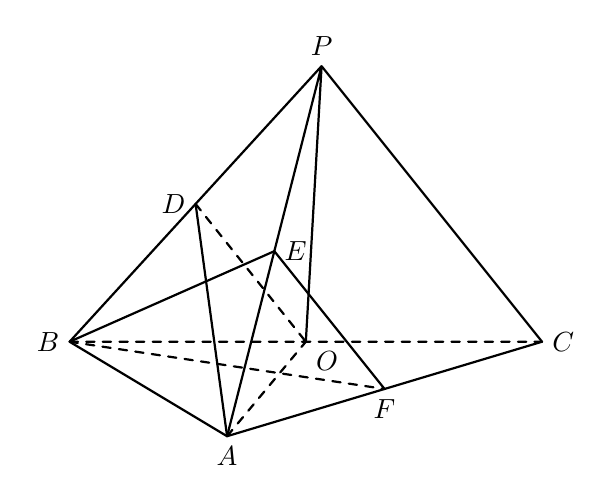
\begin{tikzpicture}[line cap=round,line join=round,line width=0.8pt]
  \coordinate (A) at (0,0);
  \coordinate (B) at (-2,1.2);
  \coordinate (C) at (4,1.2);
  \coordinate (P) at (1.2,4.7);
  \coordinate (D) at (-0.4,2.95);
  \coordinate (E) at (0.6,2.35);
  \coordinate (O) at (1,1.2);
  \coordinate (F) at (2,0.6);

  \draw (P)--(A) (P)--(B) (P)--(C) (P)--(O) (A)--(B) (A)--(C);
  \draw[dashed] (B)--(C) (A)--(O) (D)--(O) (B)--(F);
  \draw (A)--(D) (B)--(E) (E)--(F);

  \node[above] at (P) {$P$};
  \node[left] at (B) {$B$};
  \node[right] at (C) {$C$};
  \node[below] at (A) {$A$};
  \node[left] at (D) {$D$};
  \node[right] at (E) {$E$};
  \node[below right] at (O) {$O$};
  \node[below] at (F) {$F$};
\end{tikzpicture}
\end{center}
\nopagebreak[4]
(1) 证明：$EF\parallel$ 平面 $ADO$；

(2) 证明：平面 $ADO\perp$ 平面 $BEF$；

(3) 求二面角 $D-AO-C$ 的正弦值．

\Needspace{4\baselineskip}
\textbf{解析}

\Needspace{5\baselineskip}
设 $B=(0,0,0)$、$A=(2,0,0)$、$C=(0,2\sqrt2,0)$。由 $PB=PC$ 知 $P$ 的 $y$ 坐标为 $\sqrt2$；再由 $PB^2=6$ 得 $P=(u,\sqrt2,v)$ 且 $u^2+v^2=4$。于是

\nopagebreak[4]
\[
D=(u/2,\sqrt2/2,v/2),\qquad O=(0,\sqrt2,0).
\]

\Needspace{5\baselineskip}
把 $AD^2=5DO^2$ 代入，并用 $u^2+v^2=4$ 化简，得 $u=-1$，故 $v^2=3$。经坐标系关于底面反射可取 $v=\sqrt3$，所以 $P=(-1,\sqrt2,\sqrt3)$，且

\nopagebreak[4]
\[
D=(-1/2,\sqrt2/2,\sqrt3/2),\qquad E=(1/2,\sqrt2/2,\sqrt3/2).
\]

\Needspace{5\baselineskip}
由 $F\in AC$，写 $F=A+t(C-A)$。条件 $BF\perp AO$ 给出

\nopagebreak[4]
\[
F\cdot(O-A)=0\quad\Longrightarrow\quad -4+8t=0,
\]

所以 $t=1/2$、$F=(1,\sqrt2,0)$。

\gksubpart{(1) 证明线面平行}

\Needspace{5\baselineskip}
(1) 直接计算

\nopagebreak[4]
\[
\overrightarrow{EF}=(1/2,\sqrt2/2,-\sqrt3/2)
=\overrightarrow{AO}-\overrightarrow{AD}.
\]

右侧是平面 $ADO$ 内两方向向量的线性组合，故 $EF$ 平行于平面 $ADO$。

\gksubpart{(2) 证明两平面垂直}

\Needspace{5\baselineskip}
(2) 平面 $ADO$ 的法向量可取

\nopagebreak[4]
\[
n_1=\overrightarrow{AO}\times\overrightarrow{AD}
=(\sqrt6/2,\sqrt3,3\sqrt2/2).
\]

\Needspace{5\baselineskip}
平面 $BEF$ 的法向量可取

\nopagebreak[4]
\[
n_2=\overrightarrow{BE}\times\overrightarrow{BF}
=(-\sqrt6/2,\sqrt3/2,0).
\]

二者点积为 $-6/4+3/2=0$，故两平面法向量垂直，平面 $ADO\perp$ 平面 $BEF$。

\gksubpart{(3) 求二面角正弦值}

\Needspace{5\baselineskip}
(3) 因 $O\in BC$，平面 $AOC$ 与底面 $ABC$ 相同，法向量可取 $k=(0,0,1)$。有 $|n_1|=3$，且

\nopagebreak[4]
\[
|n_1\times k|=\sqrt{(\sqrt6/2)^2+(\sqrt3)^2}=\frac3{\sqrt2}.
\]

所以两平面的夹角正弦为 $|n_1\times k|/(|n_1||k|)=1/\sqrt2=\sqrt2/2$，即二面角 $D-AO-C$ 的正弦值。

\gkanswer{答案（1）：见解析版}

\gkanswer{答案（2）：见解析版}

\gkanswer{答案（3）：二面角 $D-AO-C$ 的正弦值为 $\dfrac{\sqrt2}{2}$。}

\end{answer}
\begin{answer}
\gksolhead{20}{}

\textbf{题目}：

已知椭圆 $C:\dfrac{y^2}{a^2}+\dfrac{x^2}{b^2}=1\ (a>b>0)$ 的离心率为 $\dfrac{\sqrt5}{3}$，点 $A(-2,0)$ 在 $C$ 上．

(1) 求 $C$ 的方程；

(2) 过点 $(-2,3)$ 的直线交 $C$ 于 $P\text{，}Q$ 两点，直线 $AP\text{，}AQ$ 与 $y$ 轴的交点分别为 $M\text{，}N$，证明：线段 $MN$ 的中点为定点．

\Needspace{4\baselineskip}
\textbf{解析}

\gksubpart{(1) 求椭圆方程}

\Needspace{5\baselineskip}
(1) 由 $A(-2,0)$ 在椭圆上，得 $4/b^2=1$，所以 $b=2$。离心率满足

\nopagebreak[4]
\[
\frac{c^2}{a^2}=1-\frac{b^2}{a^2}=\frac59,
\]

故 $b^2/a^2=4/9$，由 $b=2$ 得 $a=3$，方程为 $y^2/9+x^2/4=1$。

\gksubpart{(2) 证明弦中点为定点}

\Needspace{5\baselineskip}
(2) 设过 $(-2,3)$ 的直线斜率为 $k$，令 $s=x+2$，则直线为 $y=3+ks$，椭圆代入后得

\nopagebreak[4]
\[
\left(\frac{k^2}{9}+\frac14\right)s^2+\left(\frac{2k}{3}-1\right)s+1=0.
\]

\Needspace{5\baselineskip}
设两交点的 $s$ 坐标为 $s_1,s_2$。韦达定理给出

\nopagebreak[4]
\[
\frac1{s_1}+\frac1{s_2}
=\frac{s_1+s_2}{s_1s_2}
=1-\frac{2k}{3}.
\]

\Needspace{5\baselineskip}
连结 $A=(-2,0)$ 与对应交点的直线斜率分别为 $m_i=(3+ks_i)/s_i=3/s_i+k$，于是

\nopagebreak[4]
\[
m_1+m_2=3\left(1-\frac{2k}{3}\right)+2k=3.
\]

过 $A$ 且斜率为 $m_i$ 的直线在 $y$ 轴上的截距为 $2m_i$，两截距之和恒为 $6$，故 $MN$ 的中点恒为 $(0,3)$。

\gkanswer{答案（1）：$\dfrac{y^2}{9}+\dfrac{x^2}{4}=1$。}

\gkanswer{答案（2）：线段 $MN$ 的中点为定点 $(0,3)$。}

\end{answer}
\begin{answer}
\gksolhead{21}{}

\textbf{题目}：

已知函数 $f(x)=\left(\dfrac1x+a\right)\ln(1+x)$．

(1) 当 $a=-1$ 时，求曲线 $y=f(x)$ 在点 $(1\text{，}f(1))$ 处的切线方程；

(2) 是否存在 $a\text{，}b$，使得曲线 $y=f\left(\dfrac1x\right)$ 关于直线 $x=b$ 对称？若存在，求 $a\text{，}b$；若不存在，说明理由；

(3) 若 $f(x)$ 在 $(0,+\infty)$ 存在极值点，求 $a$ 的取值范围．

\Needspace{4\baselineskip}
\textbf{解析}

\gksubpart{(1) 求切线方程}

\Needspace{5\baselineskip}
(1) 求导得

\nopagebreak[4]
\[
f'(x)=-\frac{\ln(1+x)}{x^2}+\frac{1/x+a}{1+x}.
\]

当 $a=-1$、$x=1$ 时，$f(1)=0$、$f'(1)=-\ln2$。切线为 $y=-(\ln2)(x-1)$。

\gksubpart{(2) 求对称参数}

\Needspace{5\baselineskip}
(2) 令 $g(x)=f(1/x)=(x+a)\ln(1+1/x)$。由 $1/x>-1$ 且 $1/x\ne0$，$g$ 的定义域为 $(-\infty,-1)\cup(0,+\infty)$，两段的边界 $-1$、$0$ 关于对称轴的中点是 $b=-1/2$。对任意 $x>0$，

\nopagebreak[4]
\[
g(-1-x)=(x+1-a)\ln(1+1/x).
\]

它与 $g(x)=(x+a)\ln(1+1/x)$ 恒等当且仅当 $a=1/2$。因此存在所求参数，且 $a=1/2,b=-1/2$。

\gksubpart{(3) 判断极值点存在范围}

\Needspace{5\baselineskip}
(3) 对 $x>0$，

\nopagebreak[4]
\[
f'(x)=\frac{H(x)}{x^2(1+x)},\qquad
H(x)=x+ax^2-(1+x)\ln(1+x).
\]

\Needspace{5\baselineskip}
又

\nopagebreak[4]
\[
H(0)=H'(0)=0,\quad H'(x)=2ax-\ln(1+x),\quad H''(x)=2a-\frac1{1+x}.
\]

若 $a\leqslant0$，则 $H'(x)<0$，$H(x)<0$，导数无零点。若 $a\geqslant1/2$，则 $H''(x)>0$ 对 $x>0$ 成立，进而 $H'(x)>0$、$H(x)>0$，也无零点。若 $0<a<1/2$，$H''$ 恰从负变正一次，于是 $H'$ 先减后增并仅有一个正零点；$H$ 从 $0$ 先降为负，再增至 $+\infty$，故有唯一正零点，且 $f'$ 在该点由负变正，存在极小值点。所求范围为 $0<a<1/2$。

\gkanswer{答案（1）：$y=-(\ln2)(x-1)$。}

\gkanswer{答案（2）：存在，$a=\dfrac12\text{，}b=-\dfrac12$。}

\gkanswer{答案（3）：$0<a<\dfrac12$。}

\end{answer}
\begin{answer}
\gksolhead{22}{}

\textbf{题目}：

在直角坐标系 $xOy$ 中，以坐标原点为极点，$x$ 轴正半轴为极轴建立极坐标系，曲线 $C_1$ 的极坐标方程为 $\rho=2\sin\theta\ \left(\dfrac\pi4\leqslant\theta\leqslant\dfrac\pi2\right)$．曲线 $C_2:\begin{cases}x=2\cos\alpha,\\y=2\sin\alpha,\end{cases}\ (\alpha\text{ \text{为参数}},\ \dfrac\pi2<\alpha<\pi)$．

(1) 写出 $C_1$ 的直角坐标方程；

(2) 若直线 $y=x+m$ 既与 $C_1$ 没有公共点，也与 $C_2$ 没有公共点，求 $m$ 的取值范围．

\Needspace{4\baselineskip}
\textbf{解析}

\gksubpart{(1) 化为直角坐标方程}

\Needspace{5\baselineskip}
(1) 由 $x=\rho\cos\theta$、$y=\rho\sin\theta$ 和 $\rho=2\sin\theta$，得

\nopagebreak[4]
\[
x^2+y^2=\rho^2=2\rho\sin\theta=2y.
\]

角度范围对应圆 $x^2+(y-1)^2=1$ 上从 $(1,1)$ 到 $(0,2)$ 的圆弧，即 $0\leqslant x\leqslant1$、$1\leqslant y\leqslant2$ 的那一段。

\gksubpart{(2) 求参数范围}

(2) 直线 $y=x+m$ 与曲线相交等价于曲线上 $y-x=m$。

\Needspace{5\baselineskip}
对 $C_1$，

\nopagebreak[4]
\[
m=2\sin\theta(\sin\theta-\cos\theta),\qquad \frac\pi4\leqslant\theta\leqslant\frac\pi2.
\]

此函数从 $0$ 单调增至 $2$，值域为 $[0,2]$。

\Needspace{5\baselineskip}
对 $C_2$，

\nopagebreak[4]
\[
m=2(\sin\alpha-\cos\alpha),\qquad \frac\pi2<\alpha<\pi.
\]

\Needspace{5\baselineskip}
其端点极限均为 $2$，在 $\alpha=3\pi/4$ 处取最大值 $2\sqrt2$，值域为 $(2,2\sqrt2]$。所以与两曲线都无交点时，

\nopagebreak[4]
\[
m\notin[0,2]\cup(2,2\sqrt2],
\]

即 $m\in(-\infty,0)\cup(2\sqrt2,+\infty)$。

\gkanswer{答案（1）：$x^2+y^2=2y$，取满足 $0\leqslant x\leqslant1$、$1\leqslant y\leqslant2$ 的圆弧。}

\gkanswer{答案（2）：$m\in(-\infty,0)\cup(2\sqrt2,+\infty)$。}

\end{answer}
\begin{answer}
\gksolhead{23}{}

\textbf{题目}：

已知 $f(x)=2|x|+|x-2|$．

(1) 求不等式 $f(x)\leqslant6-x$ 的解集；

(2) 在直角坐标系 $xOy$ 中，求不等式组 $\begin{cases}f(x)\leqslant y,\\x+y-6\leqslant0\end{cases}$ 所确定的平面区域的面积．

\Needspace{4\baselineskip}
\textbf{解析}

\gksubpart{(1) 求不等式解集}

\Needspace{5\baselineskip}
(1) 分段表示

\nopagebreak[4]
\[
f(x)=\begin{cases}
2-3x,&x<0,\\
x+2,&0\leqslant x\leqslant2,\\
3x-2,&x>2.
\end{cases}
\]

分别代入 $f(x)\leqslant6-x$：第一段得 $x\geqslant-2$，第二段得 $x\leqslant2$，第三段得 $x\leqslant2$（与 $x>2$ 不相容）。合并得解集 $[-2,2]$。

\gksubpart{(2) 求平面区域面积}

\Needspace{5\baselineskip}
(2) 区域在 $f(x)\leqslant y\leqslant6-x$ 之间，$x$ 范围正是 $[-2,2]$。分段积分：

\nopagebreak[4]
\[
\begin{aligned}
S&=\int_{-2}^0\bigl[(6-x)-(2-3x)\bigr]dx
+\int_0^2\bigl[(6-x)-(x+2)\bigr]dx\\
&=\int_{-2}^0(4+2x)dx+\int_0^2(4-2x)dx=4+4=8.
\end{aligned}
\]

\gkanswer{答案（1）：$[-2,2]$。}

\gkanswer{答案（2）：$8$。}

\end{answer}